% Template Name: NR Presentation Template
% Author: Magne Aldrin, Anders Løland, and Trenton Schulz
% License: LaTeX Project Public License 1.3c (LPPL)
\documentclass[14pt,aspectratio=169,t]{beamer}
\usepackage{graphicx}
\usepackage{xcolor}
\usepackage{tikz}
\usepackage{paralist}
\usepackage{caption}
\usepackage[british]{babel}


% Use the same font as the Powerpoint template. To get better
% consistency with math, consider using Fira Math with LuaTeX (allows
% using OpenType fonts) see https://tex.stackexchange.com/a/473646
\usepackage{roboto}


\setbeamertemplate{navigation symbols}{}
\setbeamerfont{title}{size=\fontsize{20pt}{10}\selectfont}
\setbeamerfont{author}{size=\fontsize{16pt}{10}\selectfont}
\setbeamerfont{subtitle}{size=\fontsize{12pt}{10}\selectfont}
\setbeamerfont{frametitle}{size=\fontsize{20pt}{10}\selectfont}
\setbeamerfont{date}{size=\fontsize{12pt}{10}\selectfont}
\usecolortheme{dove}
%% Colors
\DefineNamedColor{named}{accent1}{rgb}{0.27,0.38,0.70}
\DefineNamedColor{named}{accent2}{rgb}{0.67,0.73,0.62}
\DefineNamedColor{named}{accent3}{rgb}{0.75,0.70,0.76}


\setbeamertemplate{frametitle}{\vspace*{0.8cm}\hspace*{0cm}\insertframetitle}
\addtobeamertemplate{navigation symbols}{}{
    \usebeamerfont{footline}%
    \usebeamercolor[fg]{footline}%
    \hspace{1em}%
%    \insertframenumber
  }
  \setlength{\parskip}{1cm}
%  \setlist[itemize]{itemsep=0.3em, topsep=0.2em}
%\setlength{\pltopsep}{0.5em}     % space above/below the list
%\setlength{\plitemsep}{0.1em}    % space between items

%% SPACING BETWEEN ITEMS FOR BEAMER
%% following lets me add length between items
%% http://tex.stackexchange.com/questions/16793/global-setting-of-spacing-between-items-in-itemize-environment-for-beamer
% \let\oldframe\frame
% \renewcommand{\frame}{
% \oldframe
% \let\olditemize\itemize
% %%\renewcommand\itemize{\olditemize\addtolength{\itemsep}{0.5\baselineskip}}
% \renewcommand\itemize{\olditemize\addtolength{\parskip}{0.5\baselineskip}} %% this affects nested list (itemize) as well
% }
\newlength{\wideitemsep}

\setlength{\wideitemsep}{\itemsep}
\addtolength{\wideitemsep}{0.00\baselineskip}
\let\olditem\item
\renewcommand{\item}{\setlength{\itemsep}{\wideitemsep}\olditem}
%%\usepackage{enumitem} %% traditional way to modify listing (itemize and enumerate) properties...but beamer has its own definition
%% NESTED LISTS
%% http://tex.stackexchange.com/questions/20654/length-between-nested-lists
\setbeamertemplate{itemize/enumerate subbody begin}{\vspace{0.1cm}}
\setbeamertemplate{itemize/enumerate subbody end}{\vspace{0.1cm}}
\setbeamertemplate{itemize/enumerate subsubbody begin}{\vspace{0.1cm}}
\setbeamertemplate{itemize/enumerate subsubbody end}{\vspace{0.1cm}}
%%\setbeamertemplate{itemize/enumerate subbody begin}{\vspace{0.5\baselineskip}}
%%\setbeamertemplate{itemize/enumerate subbody end}{\vspace{0.5\baselineskip}}
%% MORE OPTIONS http://tex.stackexchange.com/questions/11168/change-bullet-style-formatting-in-beamer\setbeamertemplate{itemize/enumerate subbody begin}{\vspace{1\baselineskip}}

\setbeamercolor{itemize item}{fg=accent1}
\setbeamercolor{itemize subitem}{fg=accent3}
\setbeamercolor{itemize subsubitem}{fg=accent2}


\begin{document}

% Title Slide
{
  \usebackgroundtemplate{
\includegraphics[width=1\paperwidth]{backgrounds/nr1.pdf}}
  \begin{frame}
    \vspace{2cm}
    \Large \textbf {Title here} \\
    \vspace{1cm}
    \normalsize Johannes Voll Kolstø, \\ \small Norwegian Computing Central\\
    \vspace{2cm}
    \small \today
  \end{frame}
}

\usebackgroundtemplate{
\includegraphics[width=1\paperwidth]{backgrounds/nr2.pdf}}

\begin{frame}{Slide title with text}
  \begin{itemize}
  \item Text level 1
    \begin{itemize}
    \item Text level 2
      \begin{itemize}
      \item Text level 3
      \end{itemize}  
    \end{itemize}  
  \end{itemize}
\end{frame}  


\begin{frame}{Slide title with text and formula}
  \begin{itemize}
  \item Text level 1
  \end{itemize}
  \begin{align*} 
    E &= m \cdot c^2\\
    x & \neq y \\
    \gamma &= G \\
  \int \sum &a^2 + b^2 = c^2
  \end{align*}
\end{frame}  


\begin{frame}{Figure xxx}
  \vspace{-0.5cm}
  \begin{center}
    \hspace{8cm}
    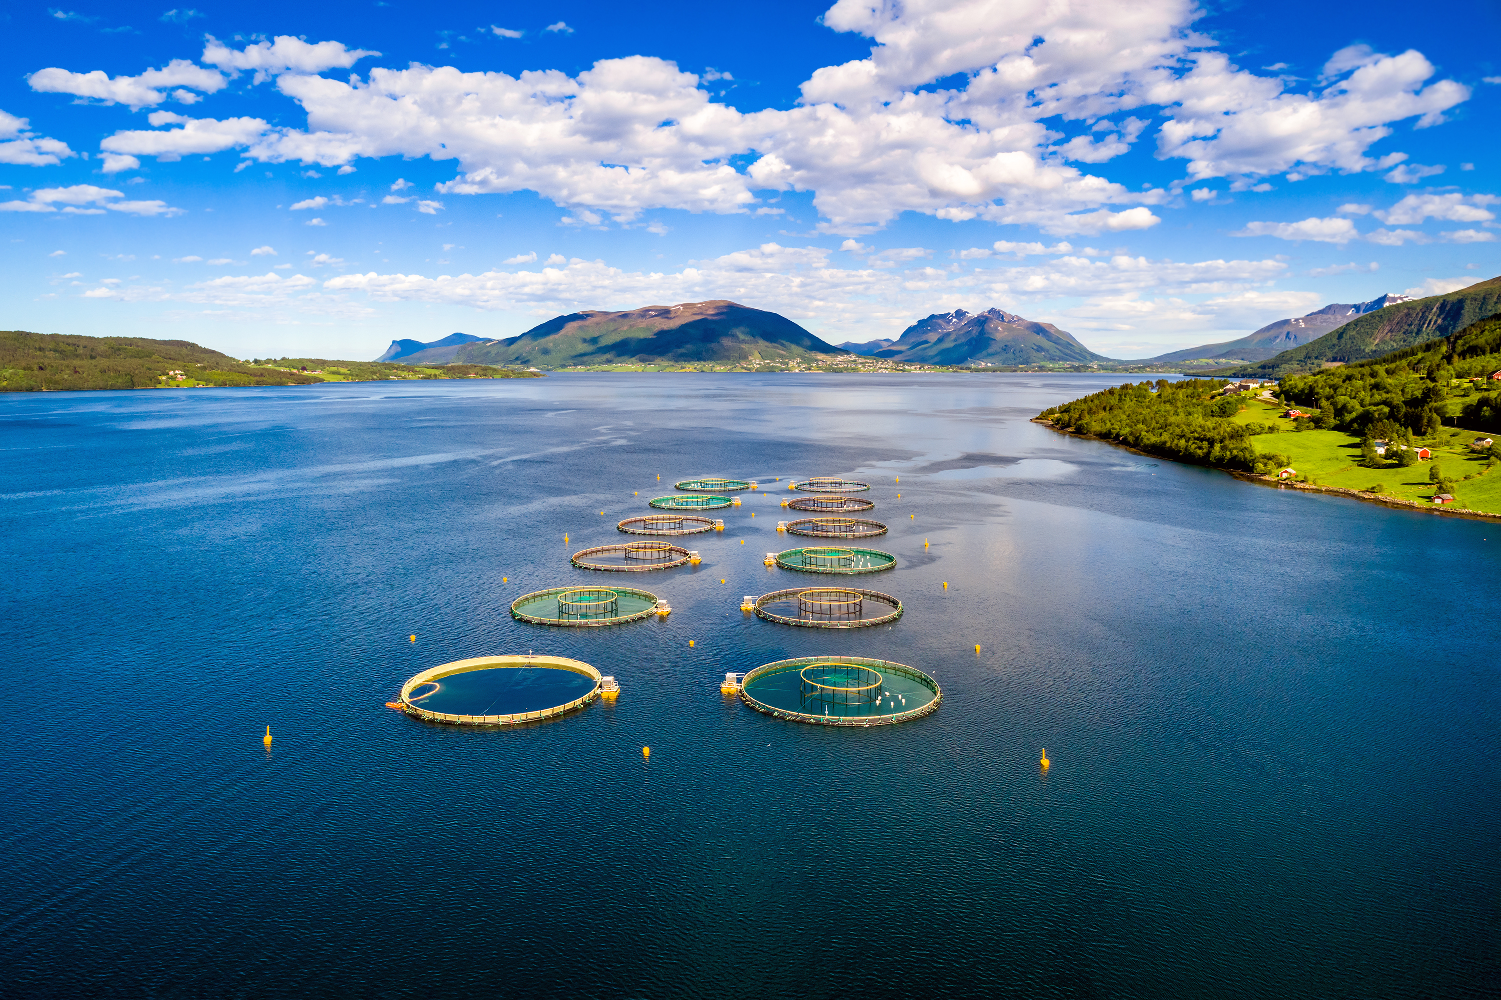
\includegraphics[width=0.60\linewidth,angle=0]{images/FishFarmAndreyArmyagov.pdf}
  \end{center}
\end{frame}  



\begin{frame}{Figure yyy}
  \begin{flushleft}
    \raisebox{0pt}[0pt][0pt]{\makebox[0pt][c]{\raisebox{-25ex}{
          \makebox[\linewidth]{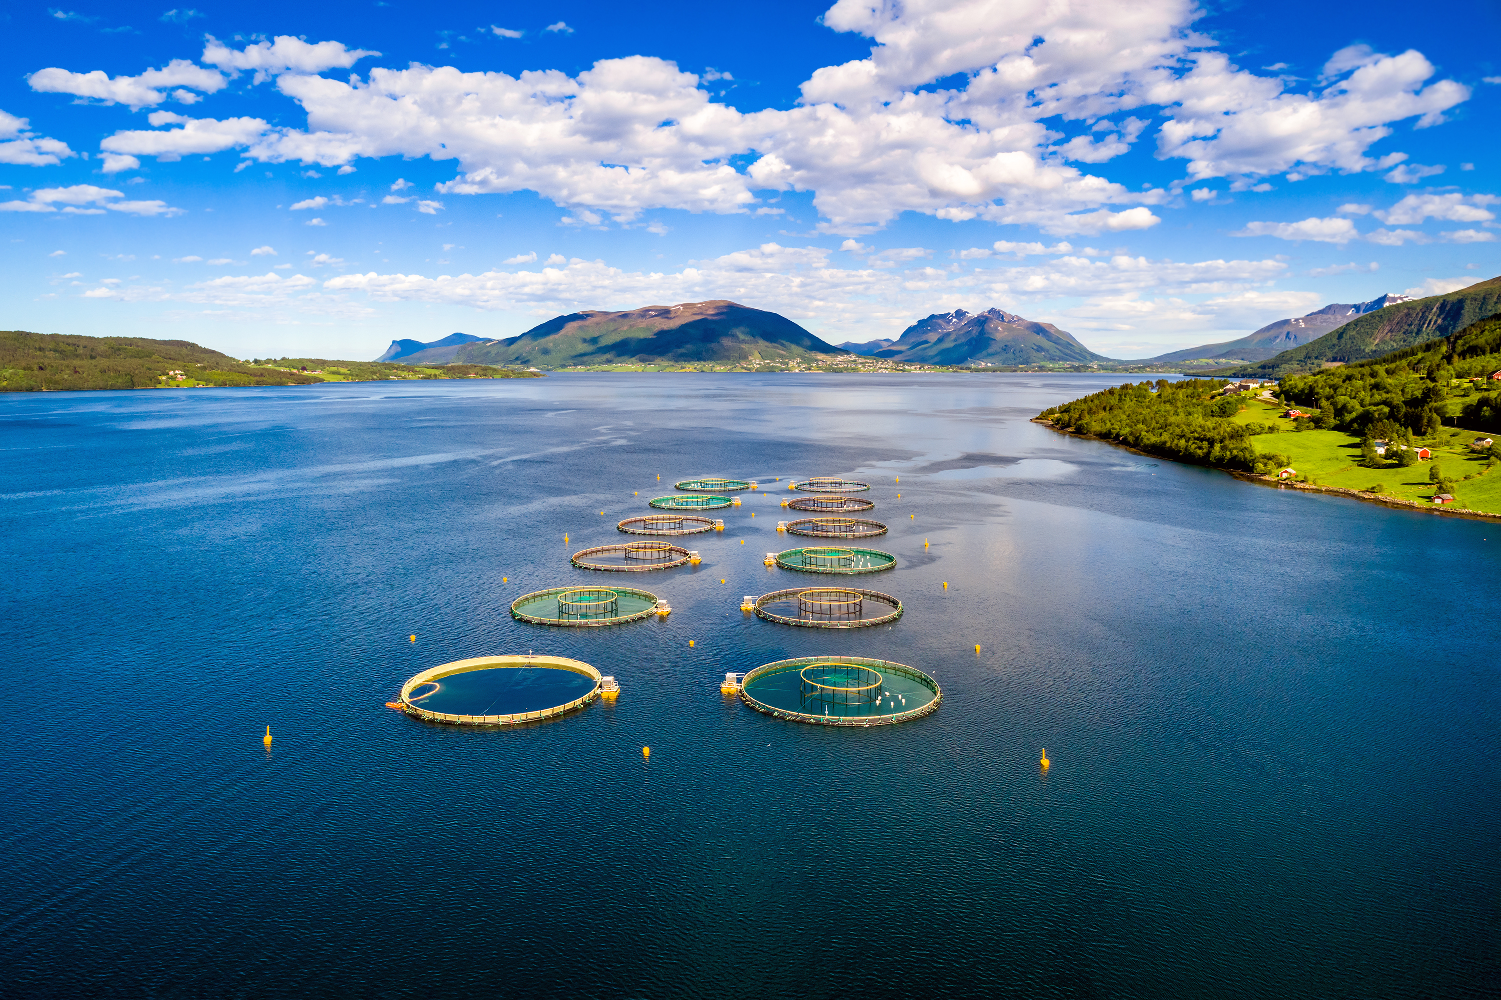
\includegraphics[type=pdf,ext=.pdf,read=.pdf,
              width=0.65\linewidth,angle=0]{images/FishFarmAndreyArmyagov}}
          \hspace{-15cm}}}} 
  \end{flushleft}
\end{frame}  


% Final slide
\usebackgroundtemplate{
\includegraphics[width=1\paperwidth]{backgrounds/nr3.pdf}}
\begin{frame}{Thank you for your attention!}
  \begin{center}
    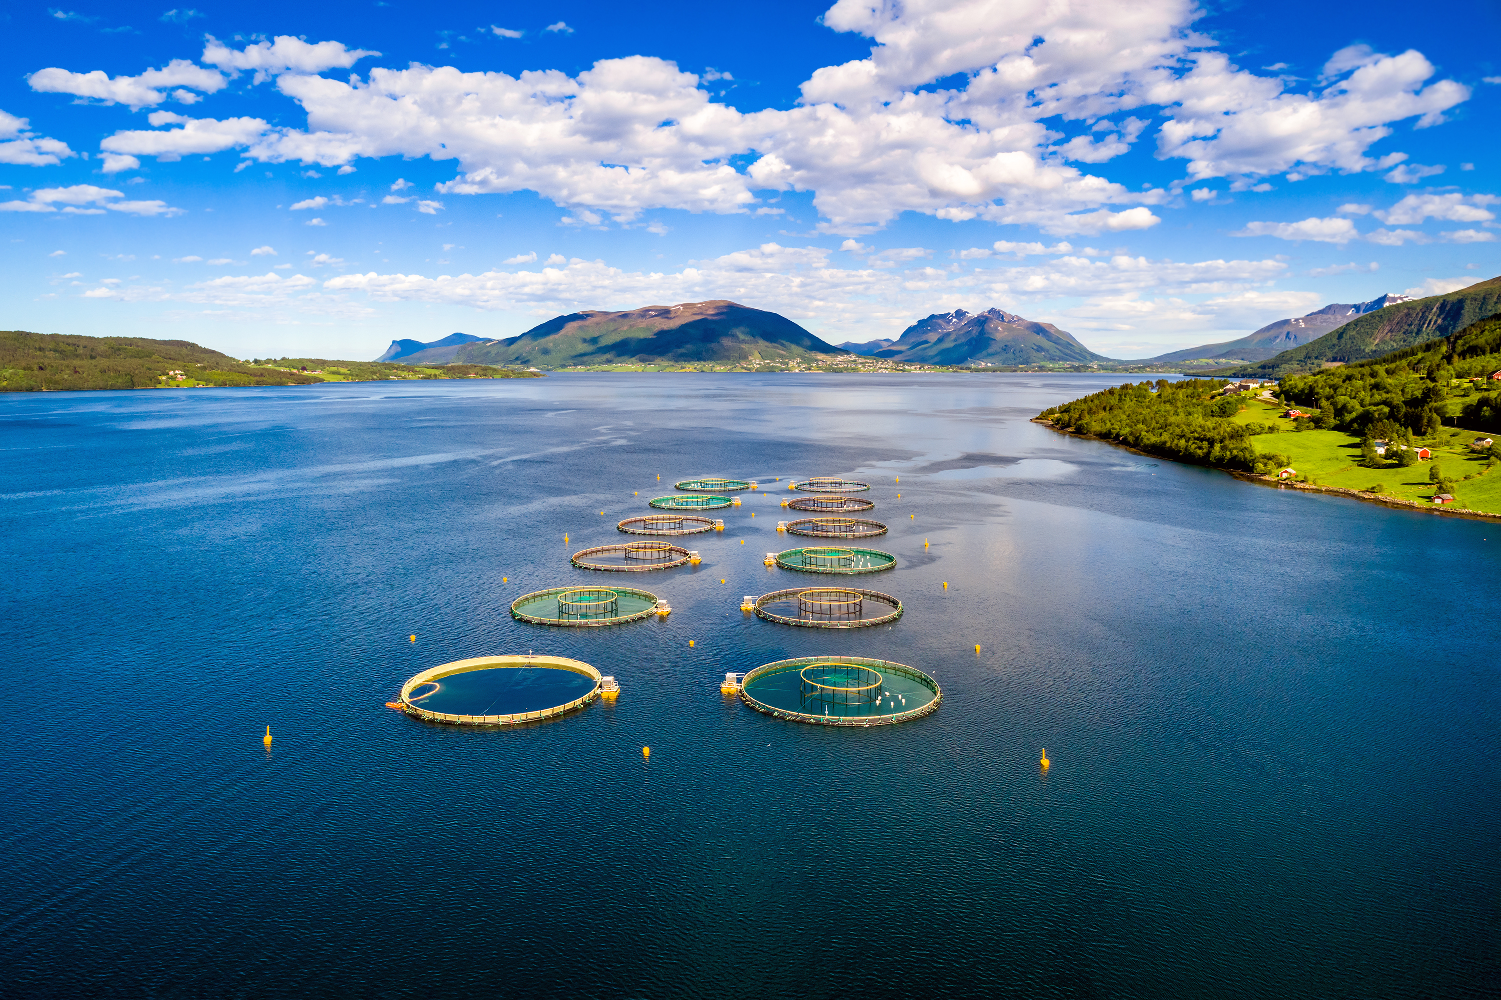
\includegraphics[width=0.60\linewidth,angle=0]{images/FishFarmAndreyArmyagov}
  \end{center}
\end{frame}

\end{document}
